\section{Catalan Objects and Dyck Paths}%
\label{sec:catalan_objects}

Dyck paths are one interpretation of the Catalan numbers.
Here, we will instead consider a more general form of Dyck Paths, which correspond to numbers in the \textit{Catalan Trapezoid}.

A Dyck path can be constructed as a $2n$ step random walk on the $\mathbb Z^2$ lattice,
starting at the origin $(0,0)$ and ending at $(n, n)$ (Figure~\ref{fig:basic_dyck}).
Each step in the walk moves one unit either along the positive $x$-axis or the positive $y$-axis.
Given these restrictions, we would obtain a 1D random walk pinned to zero  on both sides.
A Dyck path also has the additional restriction that for any position $(x, y)$ on the path, $y-x > 0$
i.e. the walk is always on one side of the diagonal.

The number of possible Dyck paths is the $n^{th}$ Catalan number --
$$C_n = \frac{1}{n+1}\cdot {2n\choose n}$$
We will attempt to support queries to a uniformly random instance of a Dyck path.
Specifically, we will want to query the position of the $i^{th}$ index.

\begin{figure}[htbp]
    \centering
    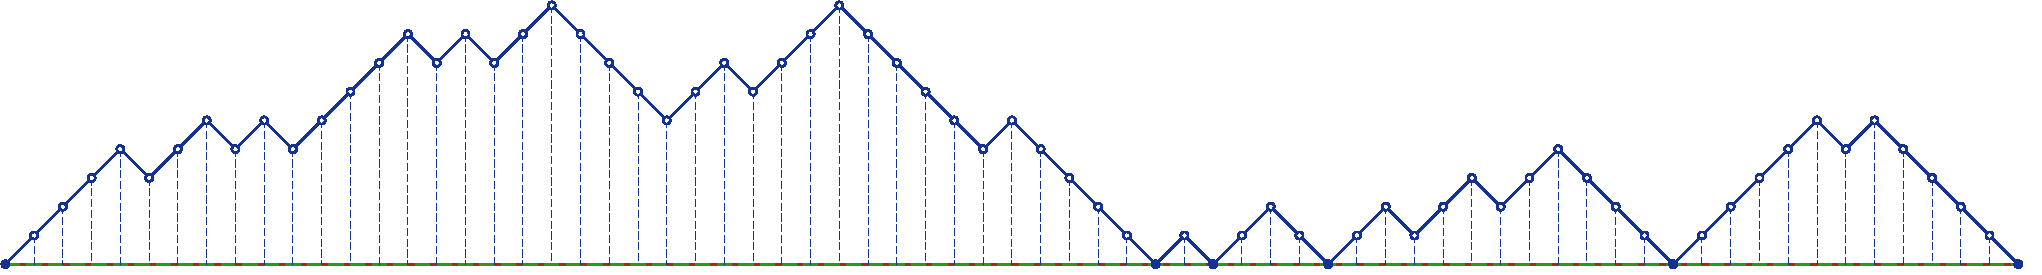
\includegraphics[width=0.7\textwidth]{dyck/basic_dyck_path.pdf}
    \caption{Simple Dyck path from $(0, 0)$ to $(20, 20)$}
    \label{fig:basic_dyck}
\end{figure}


\subsection{Catalan Trapezoids and Generalized Dyck Paths}
First, we define Catalan trapezoids as presented in \cite{trap}.
Let $C_k(n,m)$ be the $(n,m)^{th}$ entry of the Catalan trapezoid of order $k$, where $C_1(n,m)$ corresponds to the Catalan triangle.

The interpretation is as follows:
Consider a random walk from $(0,0)$ to $(m, n)$ ($n$ steps along the $y$-axis, and $m$ steps along the $x$-axis),
such that for any position $(x, y)$ along the walk, $y-x > 1-k$ (Figure~\ref{fig:complex_dyck})
i.e. the walk is always on one side of the shifted diagonal.
The total number of such paths is exactly $C_k(n,m)$.
For $k = 1$, we obtain the definition of the simple Dyck path (Figure~\ref{fig:basic_dyck}).

Now, we state a result from \cite{trap} without proof
$$
C_k(n,m)=
\begin{cases}
{n+m}\choose m &0\le m<k\\
{{n+m}\choose{m}} - {{n+m}\choose{m-k}} &k\le m\le n+k-1\\
0 &m>n+k-1
\end{cases}
$$

\begin{figure}[htbp]
    \centering
    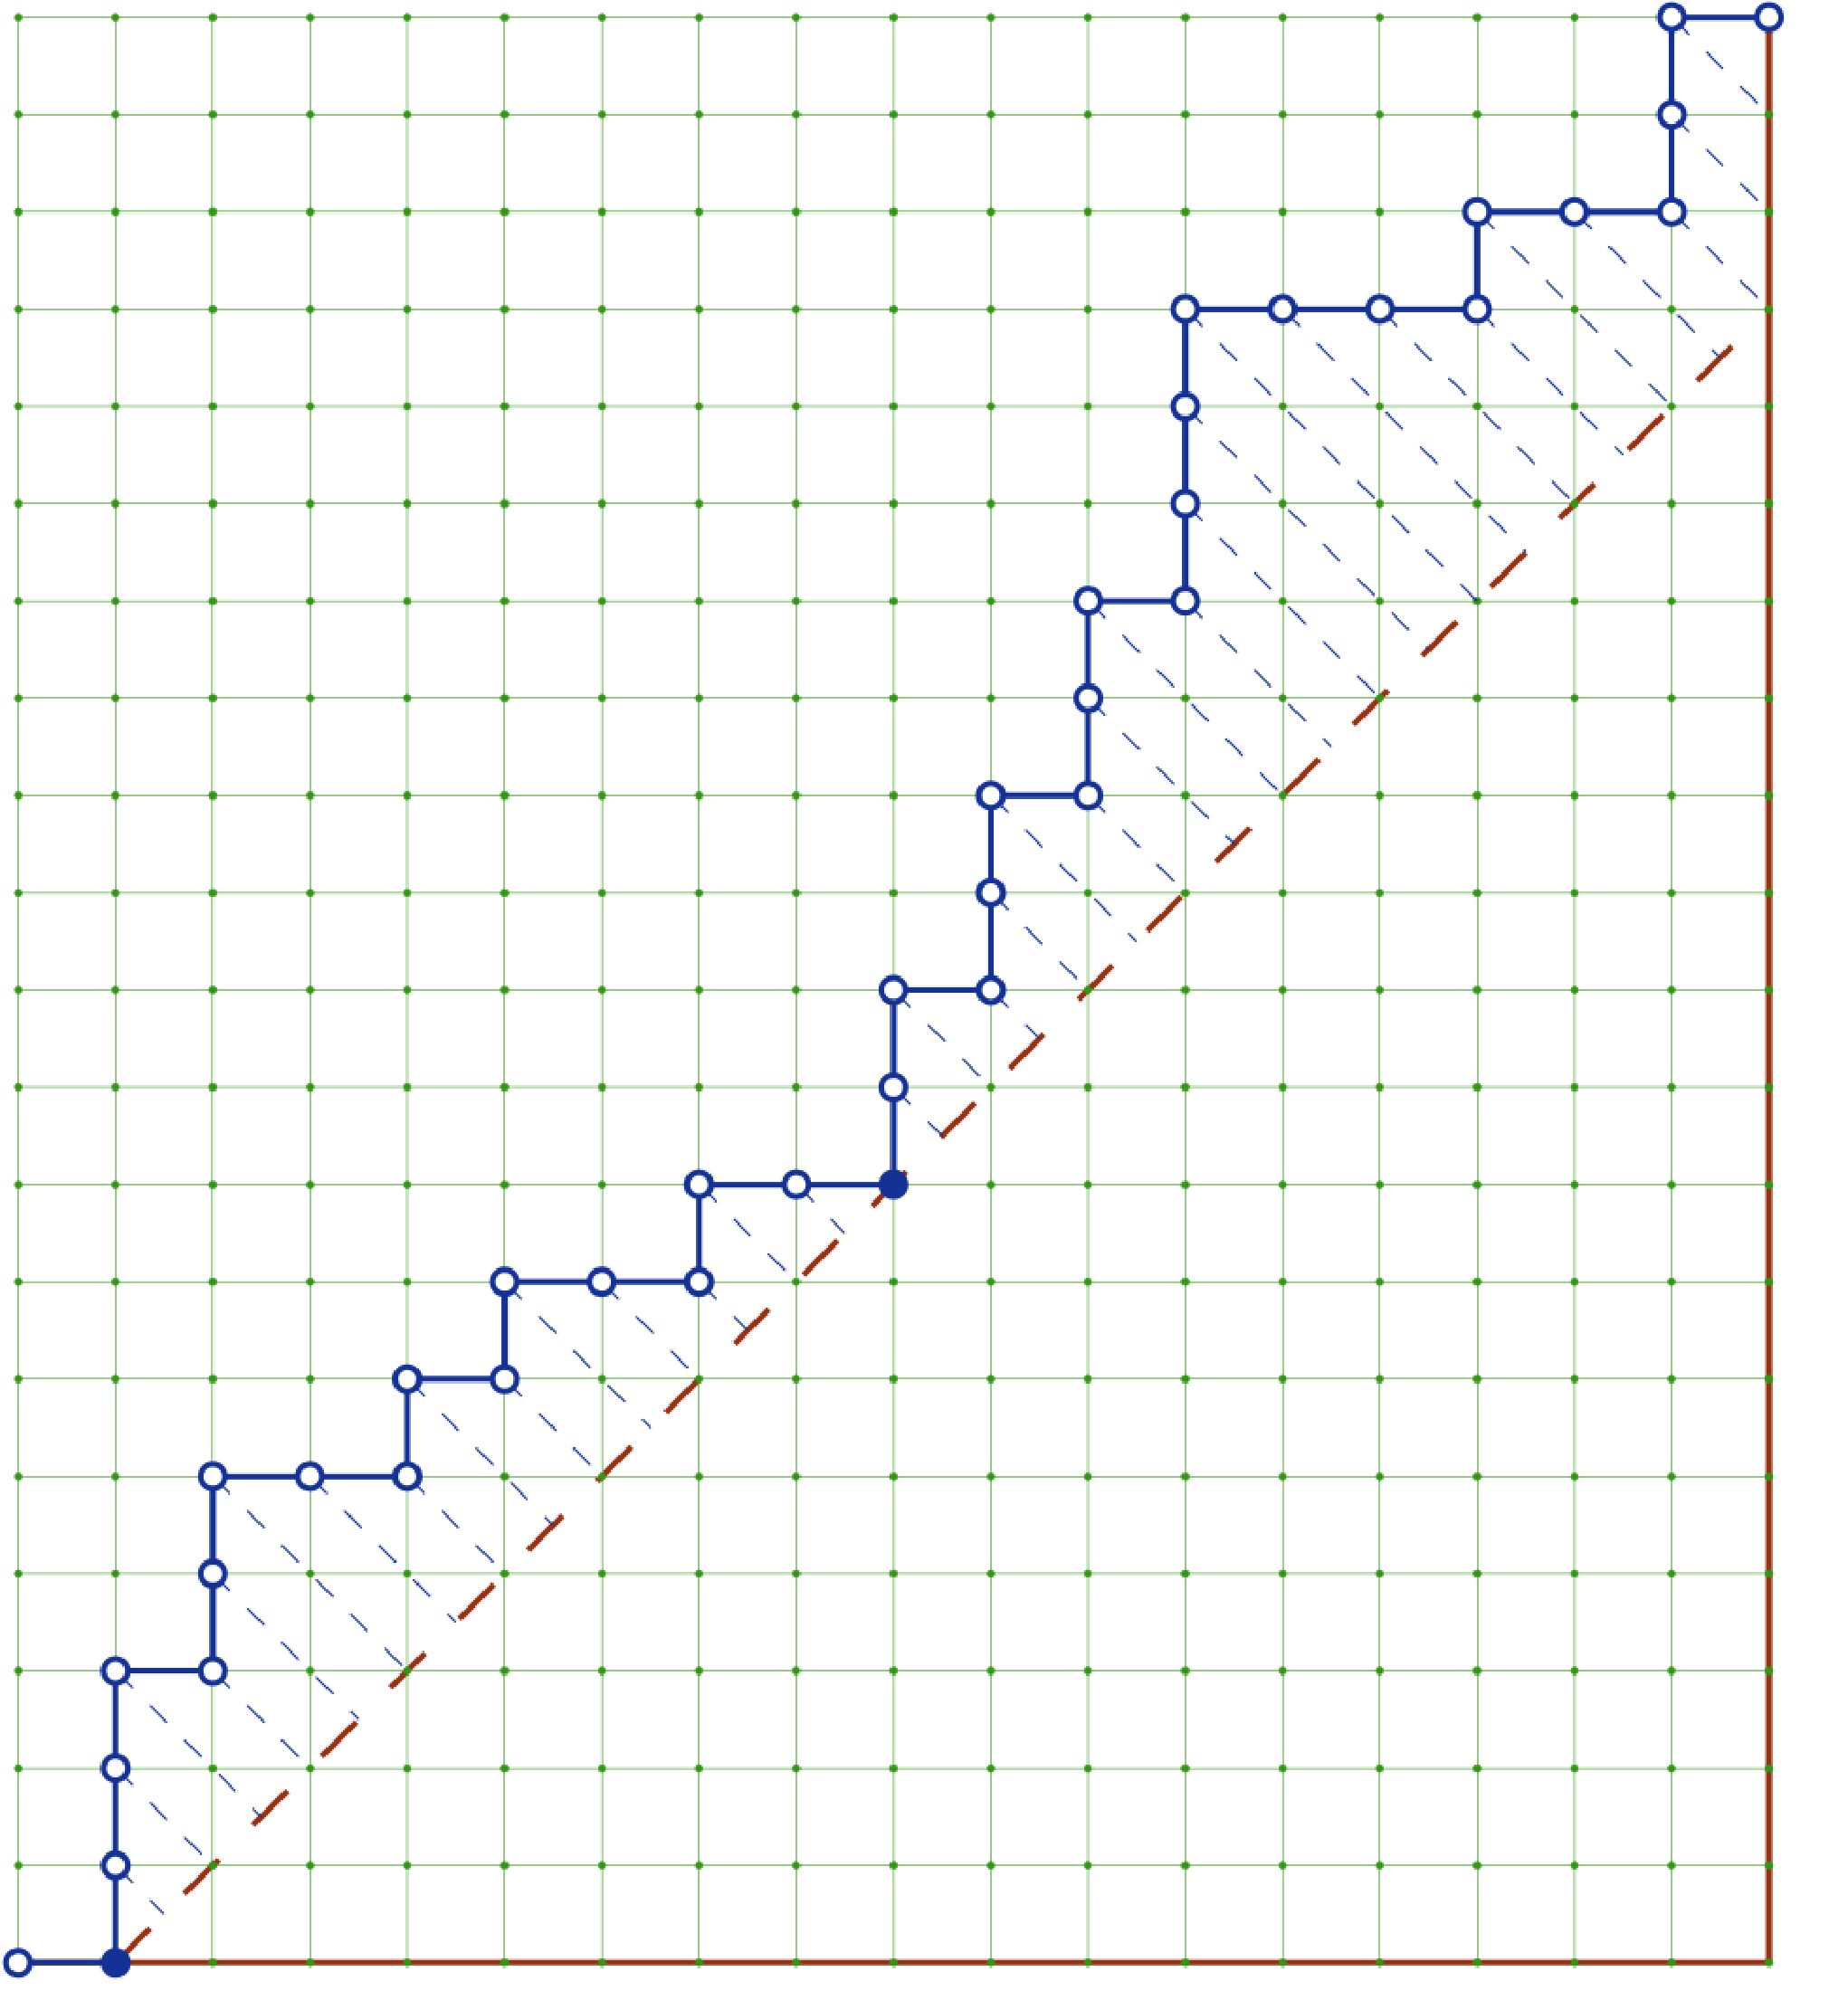
\includegraphics[width=0.7\textwidth]{dyck/complex_dyck_path.pdf}
    \caption{Complex Dyck path from $(0, 0)$ to $(18, 20)$ with $k = 2$. Notice that the diagonal is shifted.}
    \label{fig:complex_dyck}
\end{figure}

\subsection{Generating Dyck Paths}
Our general recursive step is as follows.
We consider a sequence of length $2S$ comprising of $2U$ up moves ($+1$) and $2D$ down moves ($-1$).
Additionally, the sum of any initial sequence {\color{red} prefix?} canon be less than $k-1$.
Without loss of generality, let's assume that $2D\le S$. If this were not the case,
we could simply flip the sequence and negate the elements.
This essentially means that the overall Dyck path is non-decreasing.

\begin{lemma}
$S-2D = \Bo(\log n\sqrt S) \implies U-D = \Bo(\log n\sqrt S)$
\label{lem:dyck_var0}
\end{lemma}

We want to sample the height of this path after $S$ steps.
This is the same as sampling the number of $(+1)$s that get assigned to the first half of the elements in the sequence.
We define $p_d$ as the probability that exactly $D-d$ $(-1)$s get assigned to the first half.
This means that exactly $U+d$ $(+1)$s get assigned to the first half.
Consequently, the second half will contain exactly $D+d$ $(-1)$s and $U-d$ $(+1)$s.

Let us first compute this probability.
$$
p_d = \frac{D_{left}\cdot D_{right}}{D_{tot}}
$$
Where $D_{left}$ denotes the number of valid starting sequences (first half)
and $D_{right}$ denotes the number of valid ending sequences.
Here, \textit{valid} means that each half sequence gets the appropriate number of ups and downs
and the initial sums never drop below $1-k$.
For, $D_{right}$, we will start the Dyck path from the end of the $2S$ sequence.
In this case the invalidation threshold will be a different $k'$.
This $k'$ is the final height of the $2S$ sequence. So, $k'=k+2U-2D = k+4S-2D$. We will use this fact extensively moving forward.

Also, $D_{tot}$ is the total number of possible sequences of length $2S$ , given the initial conditions.
This value is considered by constructing paths in the original direction i.e. the value of $k$ is the same.

\subsection{The Simple Case}
The problem of sampling reduces to the binomial sampling case when $k > \mathcal{O}(\log n)\sqrt S$ for some constant $c$.
In this case, the we can simply approximate the probability as
$$
\frac{{{S}\choose{D-d}}\cdot{{S}\choose{D+d}}}{{{2S}\choose{2D}}}
$$
This is because the random paths will not have initial sums less than $1-k$ with high probability.
Note that this uses the assumption that we have an increasing path.

\subsection{Path Segments Close to Zero}
The problem arises when we $k <\mathcal{O}(\log n)\sqrt{S}$. In this case we need to compute the actual probability,
Using the formula from \cite{trap}, we find that.
{\scriptsize
    \begin{align}
        D_{left} = {{S}\choose{D-d}}-{{S}\choose{D-d-k}}
        &&D_{right} = {{S}\choose{U-d}}-{{S}\choose{U-d-k'}}
        &&D_{tot} = {{2S}\choose{2D}}-{{2S}\choose{2D-k}}
    \end{align}
}
Here, $k' = k+2U-2D$, and so $k' = \Bo(\log n)\sqrt S$ (using Lemma~\ref{lem:dyck_var0}).

The final distribution we wish to sample from is given by $\{p_d\}_d$ where $p_d = \frac{D_{left}\cdot D_{right}}{D_{tot}}$.
To acieve this, we will use the following Lemma from \cite{huge}.
\begin{lemma}
\label{lem:huge}
Let $\{p_i\}$ and $\{q_i\}$ be distributions satisfying the following conditions
\begin{enumerate}
    \item There is a poly-time algorithm to approximate $p_i$ and $q_i$ up to $\pm n^{-2}$
    \item Generating an index $i$ according to $q_i$ is closely implementable.
    \item There exists a $poly(log n)$-time recognizable set $S$ such that
    \begin{itemize}
        \item $1-\SL{i\in S}{} p_i$ is negligible
        \item There exists a constant $c$ such that for every $i$, it holds that $p_i\le \log^{\mathcal{O}(1)} n\cdot q_i$
    \end{itemize}
\end{enumerate}
Then, generating an index $i$ according to the distribution $\{p_i\}$ is closely-implementable.
\end{lemma}

In this process, we will first disregard all values of $d$ where $|d|>\Theta(\log n\sqrt S)$.
The probability mass associated with these values can be shown to be negligible \todo{bound variance of path}.

Next, we will construct an appropriate $\{q_i\}$ and show that $p_d < \log^{\mathcal{O}(1)} n\cdot q_d$
for all $|d|<\Theta(\sqrt S)$ and some constant $c$.
We will use the following distribution
$$
q_d = \frac{{S\choose D-d}\cdot{S\choose D+d}}{{2S\choose 2D}} = \frac{{S\choose D-d}\cdot{S\choose U-d}}{{2S\choose 2D}}
$$
It is shown in \cite{huge} that this distribution is closely implementable.

First, we consider the case where $k\cdot k'\le 2U+1$.
In this case, we use loose bounds for $D_{left} < \binom{S}{D-d}$ and $D_{right} < \binom{S}{U-d}$.
We also use the following lemma (proven in Section~\ref{sec:dyck_appendix}).

\begin{restatable}{lemma}{D_tot_far_boundary}
\label{lem:D_tot_far_boundary}
When $kk' > 2U + 1$, $D_{tot} > \frac 12\cdot \binom{2S}{2D}$.
\end{restatable}

Combining the three bounds we obtain $p_d < \frac 12 q_d$.
Intuitively, in this case the dyck boundary is far away, and therefore the number of possible paths
is only a constant factor away from the number of unconstrained paths (no boundary).

The case where the boundaries are closer (i.e. $k\cdot k' \le 2U+1$) is trickier,
since the individual counts need not be close to the corresponding binomial counts.
However, in this case we can still ensure that the sampling probability is within
poly-logarithmic factors of the binomial sampling probability.
We use the following lemmas (proven in Section~\ref{sec:dyck_appendix}).

\begin{restatable}{lemma}{D_left_bound}
\label{lem:D_left_bound}
$D_{left} \le c_1 \frac{ k\cdot\log n}{\sqrt{S}}\cdot{{S}\choose{D-d}}$ for some constant $c_1$.
\end{restatable}

\begin{restatable}{lemma}{D_right_bound}
\label{lem:D_right_bound}
$D_{right} < c_2 \frac{k'\cdot log n}{\sqrt{S}}\cdot{{S}\choose{U-d}}$ for some constant $c_2$.
\end{restatable}

\begin{restatable}{lemma}{D_tot_near_boundary}
\label{lem:D_tot_near_boundary}
When $kk' \le 2U + 1$, $D_{tot} < c_3 \frac{k\cdot k'}{S}\cdot{{2S}\choose{2D}}$ for some constant $c_3$.
\end{restatable}

We can now put these lemmas together to show that $p_d/q_d \le \Theta(\log^2 n)$.
Now, we can apply Lemma~\ref{lem:huge} to sample the value of $d$,
which gives us the height of the Dyck path at the midpoint of the two given points.

\begin{theorem}
\label{thm:dyck_midpoint_sampling}
There is an algorithm that given two points at distance $a$ and $b$ (with $a < b$) along a Dyck path of length $2n$,
with the guarantee that no position between $a$ and $b$ has been sampled yet,
returns the height of the path halfway between $a$ and $b$.
Moreover, this algorithm only uses $\mathcal O(poly(\log n))$ resources.
\end{theorem}
\begin{proof}
If $b-a$ is even, we can set $S = (b-a)/2$.
Otherwise, we first sample a single step from $a$ to $a+1$, and then set $S = (b-a-1)/2$.
Since there are only two possibilities for a single step,
we can explicitly compute an approximation of the probabilities, and then sample accordingly.
Now, if $S > \Theta(\log^2 n)$ we can simply use the rejection sampling procedure described above
to obtain a $\mathcal O(poly(\log n))$ algorithm.
Otherwise, we sample each step induividually.
Since there are only $2S = \Theta(\log^2 n)$ steps, the sampling is still efficient.
\end{proof}

\begin{theorem}
\label{thm:dyck_sampling}
There is an algorithm that provides sample access to a Dyck path of length $2n$,
by answering queries of the form \func{Height}$(x)$ with the correctly sampled height of the Dyck path at position $x$
using only $\mathcal O(poly(\log n))$ resources per query.
\end{theorem}
\begin{proof}
The algorithm maintains a successor-predecessor data structure (e.g. Van Emde Boas tree)
to store all positions $x$ that have already been queried.
Each newly queried position is added to this structure.
Given a query \func{Height}$(x)$, the algorithm first finds the successor and predecessor
(say $a$ and $b$) of $x$ among the alredy queried positions.
This provides us the quarantee required to apply Theorem~\ref{thm:dyck_midpoint_sampling},
which allows us to query the height at the midpoint of $a$ and $b$.
We then binary search by updating either the successor or predecessor of $x$.
Once the interval length becomes less than $\Theta(\log^2 n)$,
we perform the full sampling (as in Theorem~\ref{thm:dyck_midpoint_sampling}) which provides us the height at position $x$.
\end{proof}


